%\documentclass{beamer}
\documentclass[aspectratio=169]{beamer}
\usepackage{transparent}
\usepackage[beamer]{shortcut}


\usepackage{animate}
\usepackage{bibentry}
\usepackage{appendixnumberbeamer}

\graphicspath{{./images/}}
\def\TikzLocation{./tikz/}
\def\tkzscl{1}

\def\onecol{}
\def\twocols{}
\def\twoblocks{}
% \def\btitle{}
\def\bimplies#1{{\centering $\Rightarrow$ #1\\}}
\def\partintro{}



\definecolor{primary}{RGB}{191,213,219}
\definecolor{secondary}{RGB}{144,106,66}
\setbeamercolor{block title}{fg=darkred}
\newcommand{\btitle}[1]{{\usebeamerfont{block title}\usebeamercolor[fg]{block title} #1}}


\setbeamertemplate{frametitle}{
  \begin{beamercolorbox}[left, leftskip=1ex,colsep*=.5em,wd=\paperwidth]{block title}
	\usebeamerfont*{frametitle}{\phantom{Gg}\hskip-3ex\insertframetitle}
  \end{beamercolorbox}
  \vskip-1em
  \begin{beamercolorbox}[wd=\paperwidth]{separation line}
    \rule{0pt}{1pt}
  \end{beamercolorbox}
}

\AtBeginSection[]
{
}


\makeatletter
\def\beamer@newblock{%
  \usebeamercolor[fg]{bibliography entry author}%
  \usebeamerfont{bibliography entry author}%
  \usebeamertemplate{bibliography entry author}%
  \def\newblock{%
    \usebeamercolor[fg]{bibliography entry title}%
    \usebeamerfont{bibliography entry title}%
    \usebeamertemplate{bibliography entry title}%
    \def\newblock{%
      \usebeamercolor[fg]{bibliography entry location}%
      \usebeamerfont{bibliography entry location}%
      \usebeamertemplate{bibliography entry location}%
      \def\newblock{%
        \usebeamercolor[fg]{bibliography entry note}%
        \usebeamerfont{bibliography entry note}%
        \usebeamertemplate{bibliography entry note}}}}%
  \leavevmode\setbox\beamer@tempbox=\hbox{}\ht\beamer@tempbox=0em\box\beamer@tempbox}
  \setbeamertemplate{bibliography entry title}{}{}

\makeatother

\definecolor{fista}{RGB}{192,192,0}
\definecolor{rcd}{RGB}{0,128,0}
\definecolor{cd}{RGB}{255, 0, 0}
\definecolor{dicod}{RGB}{0,0,255}

\usepackage[square, authoryear]{natbib}


%-----------------------------------------------------------------------------
%	CUSTOM COMANDS
%-----------------------------------------------------------------------------

\def\keypoint#1{\hfill\textcolor{gray}{#1}}
\def\mycite#1{\keypoint{\citep{#1}}}
\def\biblio{
	\nobibliography{../../library}
	\def\biblio{}
}




%\usepackage{lxfonts}

\institute{CMLA, ENS Paris-Saclay}
\author{{\bf Thomas Moreau}, Laurent Oudre, Nicolas Vayatis\\}
\title{DICOD: Distributed Coordinate Descent for Convolutional Sparse Coding}

\event{ICML 2018}
\location{Stockholm}
\def\LOGOS{\vskip-3em\includeLogos[1em]{logo_cmla, logo_ens, logo_UP13,logo_cnrs}}
\def\extraLogo{}

\date{
  Dec. 19, 2017\\[2.5ex]
  \hspace{3ex}Committee:\\[1ex]
  \noindent
  \begin{tabular}{@{}lp{7em}ll}
    Stéphanie Allassonière & Examiner &
    Alexandre Gramfort & Examiner\\
    Pierre-Paul Vidal & Examiner &
    René Vidal & Referee\\
    Stéphane Mallat & Referee &
    Julien Mairal & Referee\\
    Nicolas Vayatis & Supervisor &
    Laurent Oudre & Co-supervisor
  \end{tabular}
}

\setbeamertemplate{title page}[frame]


\begin{document}

\begin{frame}[plain]
\titlepage
\biblio{}
\end{frame}


\begin{frame}[t]{Convolutional Dictionary Learning}

	\centering
	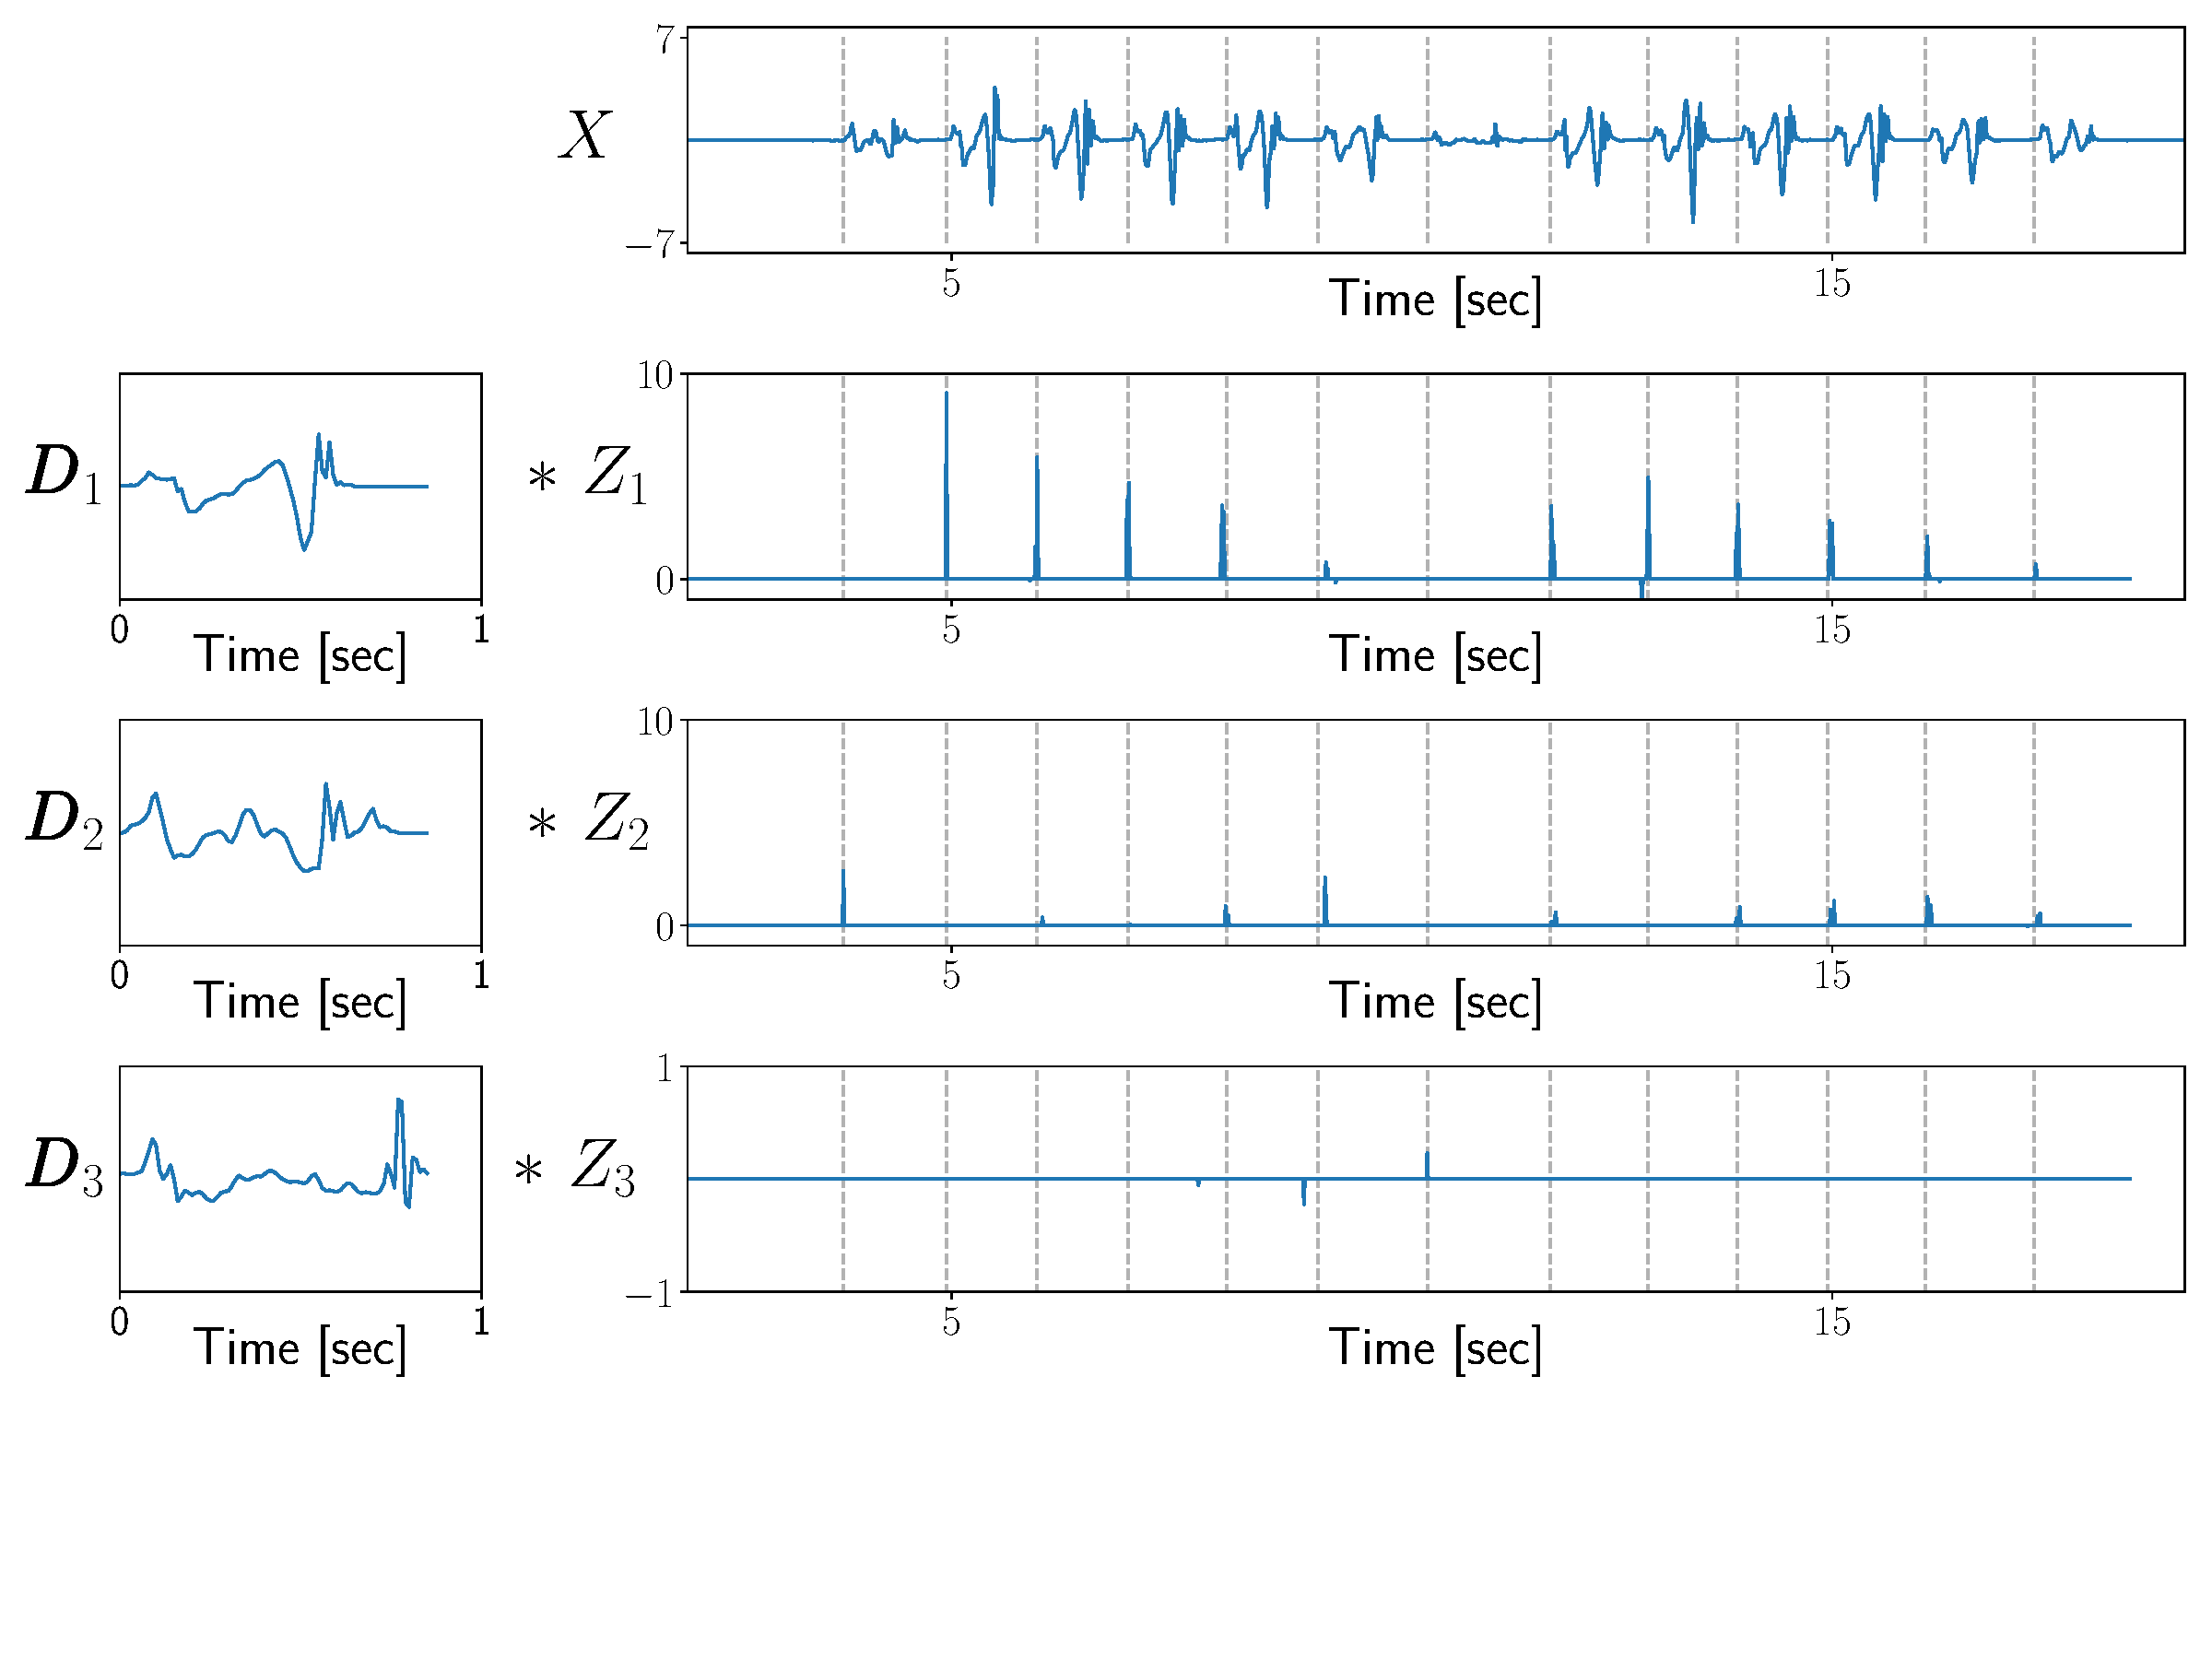
\includegraphics[width=.75\textwidth]{csc_explain}
\end{frame}




\begin{frame}[t]{Convolutional Sparse coding \phantom{)}}
$\rightarrow$ $X$ of length $T$, $\pmb D$ fixed in $\Rset^{K\times W}$; find $Z$ in $\Rset^{K\times L}$ with $L=T-W + 1$,
\[
Z^{*} = \argmin_{Z}\| X - \sum_{k=1}^K\pmb D_k *  Z_k\|_2^2
+ \lambda\| Z\|_1
\]
\vskip1em
%
\underline{\textbf{Classical Algorithms:}}\\[.5em]
\begin{itemize}%\itemsep.5em
\item Coordinate Descent ({\color{cd} CD}) \\
\mycite{Friedman2007, Kavukcuoglu2013}
\item Fast Iterative Soft-Thresholding Algorithm ({\color{fista} FISTA})\\
\mycite{Beck2009, Chalasani2013}
\item Alternated Direction Method of Multiplier (ADMM)\\
\mycite{Gabay1976, Bristow2013}
\vskip1em
\bimplies{Do not scale well with long signals $T \gg 1$.}
\end{itemize}
\end{frame}


\begin{frame}[t]{Coordinate Descent (CD)}
$\rightarrow \pmb D$ fixed, update $Z$
\[
Z^{*} = \argmin_{Z}\| X - \sum_{k=1}^K\pmb D_k *  Z_k\|_2^2
+ \lambda\| Z\|_1
\]
\vskip1em
%
\underline{\bf Coordinate Descent:}
\begin{columns}[T]
	\column{.5\textwidth}
	Select a coordinate $(k_0, t_0)$ to update.
	
	\begin{itemize}\itemindent1em
		\item Cyclic/Random updates; $\bO{1}$,
		\item Greedy updates; $\bO{KL}$.
	\end{itemize}
	\column{.5\textwidth}
	Update the value for $Z_{k_0}[t_0]$
	\begin{itemize}\itemindent1em
		\item For convolutional setting; $\mathcal O(KW)$.\\[.5em]
		\item Local operation: only impact a time segment of size $2W-1$
	\end{itemize}
\end{columns}
\vfill
\mycite{Friedman2007, Nesterov2010, Osher2009}
\end{frame}

\begin{frame}{Locally Greedy Coordinate Descent}

{\bf Key idea:} Matches CD selection complexity with update complexity.\\[2em]
\bimplies{Select the coordinate in a locally greedy fashion.}
\vskip2em
\uncover<2->{
Take the update greedily in a subsegment of the signal,
{\small\[
	\mathcal C_m = \left \{ m \left\lfloor\frac{L}{M}\right\rfloor , \dots
	(m+1) \left\lfloor\frac{L}{M}\right\rfloor -1 \right \} .\]}

This is efficient when $M = \bO{\frac{L}{W}}$ as both part of the CD algorithm have the same computational complexity $\bO{KW}$.
}
\end{frame}



\begin{frame}{Distributed Convolutional Coordinate Descent (DICOD)}
\vskip1em

$Z$ is the coding signal of length $L$.\\[.5em]
Each core $\mathcal C_m$ is responsible for the updates of a contiguous segment
{\small\[
	\mathcal C_m = \left \{ m \left\lfloor\frac{L}{M}\right\rfloor , \dots
(m+1) \left\lfloor\frac{L}{M}\right\rfloor -1 \right \} .\]}

\centering
\only<-10>{
\inputTikZ{.75}{dicod_tikz.tex}
}
%\only<11>{
%Use the {\bf structure} of convolutional LASSO to derive a parallel algorithm based on {\bf CD} with\\[1em]
%\begin{columns}[T]
%	\column{.5\textwidth}
%	\begin{itemize}
%		\item Asynchronous updates
%		\item Efficient communications
%	\end{itemize}
%	\column{.5\textwidth}
%	\begin{itemize}
%		\item No exogenous parameters
%		\item Maximal update rules
%	\end{itemize}
%\end{columns}
%}
\end{frame}



\begin{frame}{Distributed Convolutional Coordinate Descent ({\color{dicod}DICOD})}


{\bf Theoretical results:}\\[2em]
\begin{itemize}\itemsep1em
	\item \underline{Guaranteed convergence:}  We show that the interferences do not break the algorithm. even when run in an asynchronous setting
	\item \underline{Superlinear speedup:} More than twice as fast when doubling $M$.\\
	\begin{itemize}\itemsep.7em
		\item Speed-up due to the parallelization on $M$ cores.
		\item Speed-up to the complexity reduction of each iteration.
	\end{itemize}
\end{itemize}

\vskip3em


\end{frame}









\begin{frame}{Numerical convergence}

\centering
\only<1>{
	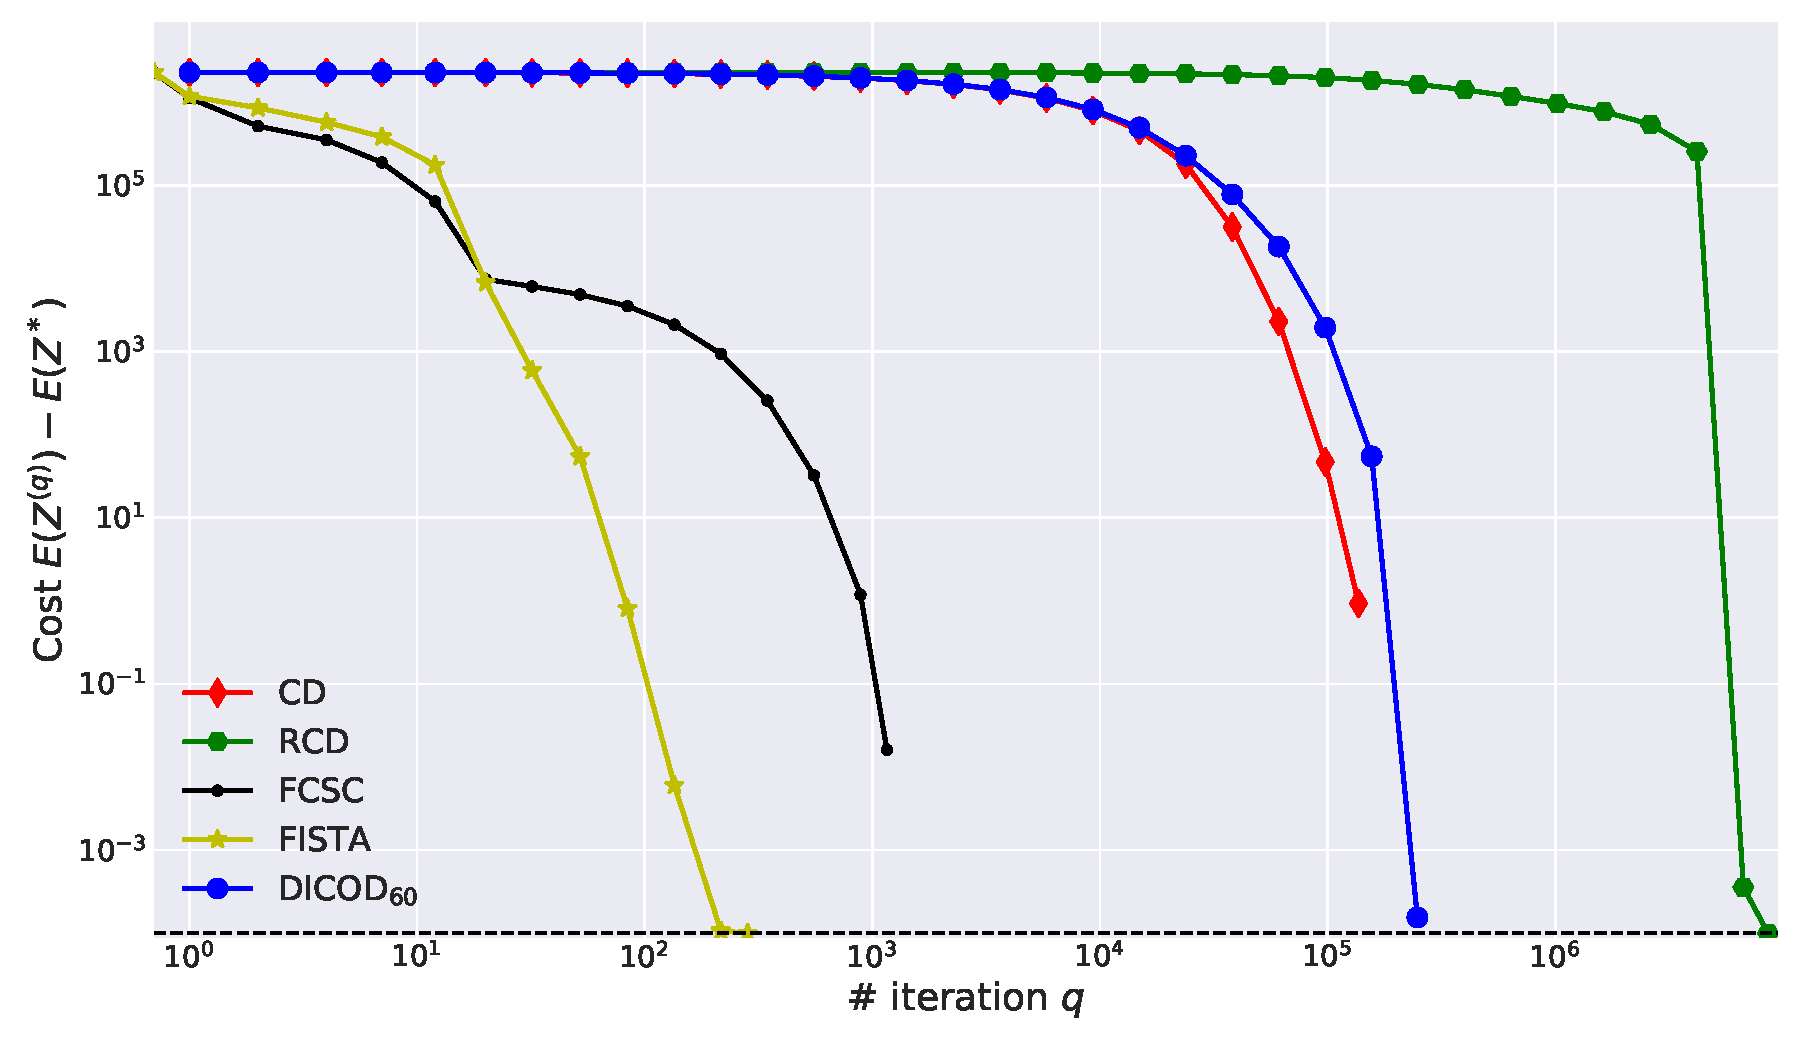
\includegraphics[width=.8\textwidth]{cost_min_seaborn_iter}\\
	\large Cost as a function of the iterations 
}

\only<2>{
	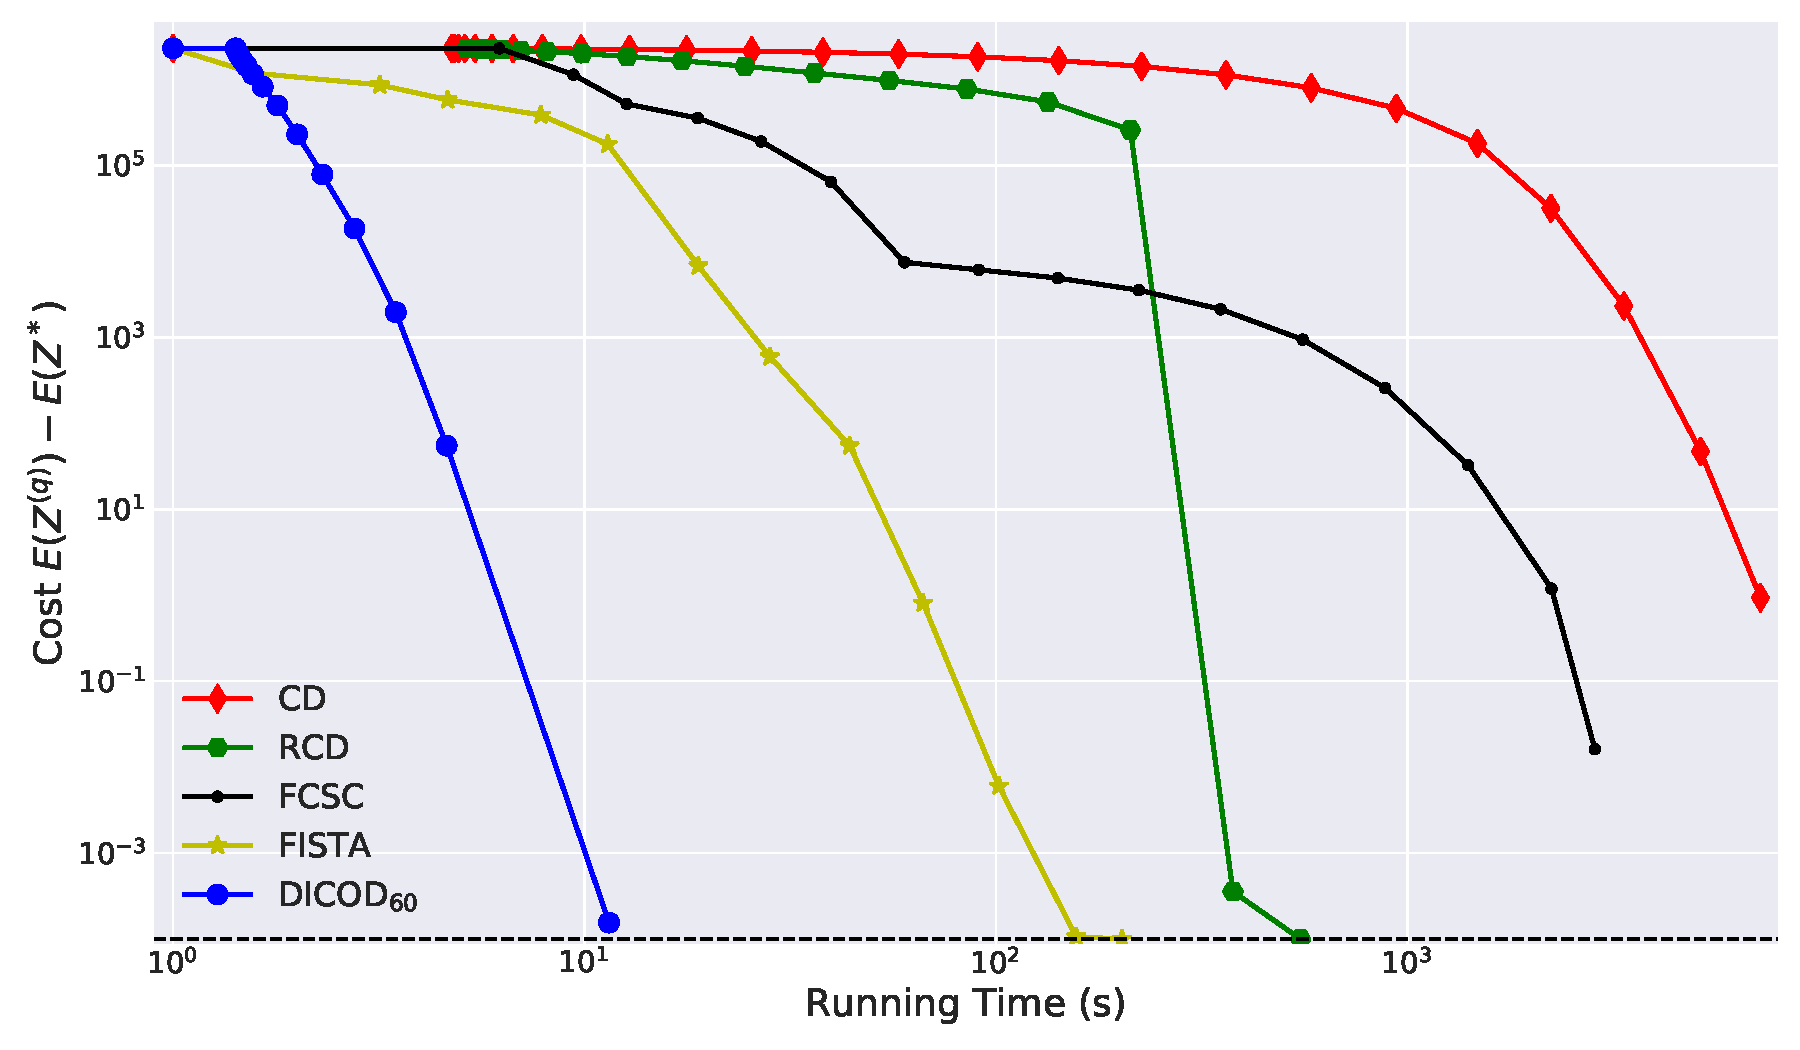
\includegraphics[width=.8\textwidth]{cost_min_seaborn_time}\\
	\large Cost as a function of the runtime
}
\end{frame}


\begin{frame}{Super-linear scaling of DICOD}
\centering
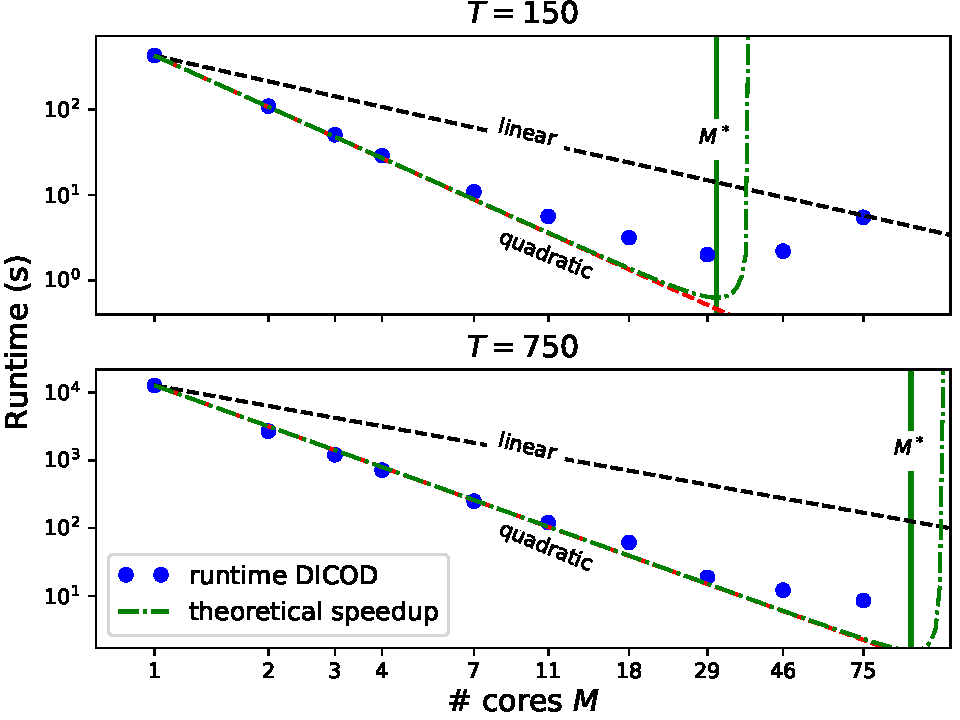
\includegraphics[width=.6\textwidth]{scaling}\\
\large Runtime as a function of the number of cores $M$
\end{frame}

\begin{frame}[t]{DICOD: Distributed Coordinate Descent for\\Convolutional  Sparse Coding}
Use the {\bf structure} of convolutional LASSO to derive a parallel algorithm based on {\bf CD} with\\[1em]
\begin{columns}[T]
	\column{.5\textwidth}
	\begin{itemize}
		\item Asynchronous updates
		\item Efficient communications
	\end{itemize}
	\column{.5\textwidth}
	\begin{itemize}
		\item No exogenous parameters
		\item Maximal update rules
	\end{itemize}
\end{columns}
\vskip2em


\includegraphics[height=.8em]{github} github.com/tommoral/dicod\hfill

\includegraphics[height=.8em]{twitter} @tomamoral {\color{gray}(note the extra 'a')}
\vskip2em
\uncover<2>{
	\begin{columns}[T]
		\column{.4\textwidth}
{\centering
	\Huge Thanks!\\[1em]
	\Large Poster\#33 tonight!\\}
\column{.05\textwidth}
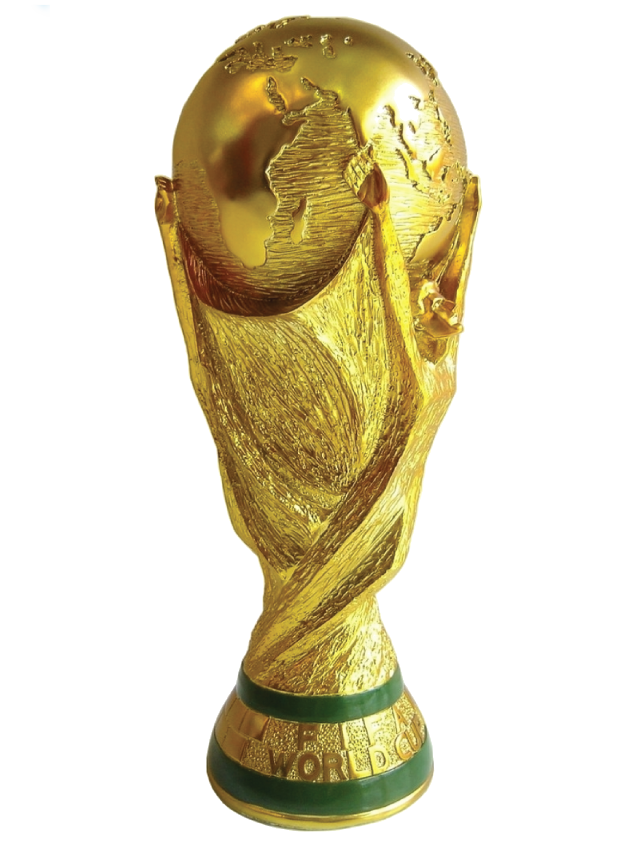
\includegraphics[height=5em]{world_cup}
\column{.3\textwidth}
\vskip1em
\centering\Large It's coming home!\\
Allez les bleus!
\column{.15\textwidth}
\vskip1em
\includegraphics[height=3em]{fr}

\end{columns}}
\end{frame}


\end{document}
